\documentclass[
	% -- opções da classe memoir -- https://www.ctan.org/pkg/memoir
	12pt,				% tamanho da fonte
	openright,			% capítulos começam em página ímpar
	                    % (insere página vazia caso preciso)
	oneside,			% caso queira imprimir em frente e verso, use twoside
	a4paper,			% tamanho do papel.
	% -- opções da classe abntex2 -- https://www.ctan.org/pkg/abntex2
	%chapter=TITLE,		% títulos de capítulos convertidos em letras maiúsculas
	%section=TITLE,		% títulos de seções convertidos em letras maiúsculas
	%subsection=TITLE,	% títulos de subseções convertidos em letras maiúsculas
	%subsubsection=TITLE,% títulos de subsubseções convertidos em letras maiúsculas
	% -- opções do pacote babel --
	english,			% idioma adicional para hifenização
	brazilian   		% para trabalhos em inglês não é necessário alterar aqui
	                    % altere o idioma após o comando \begin{document}
	]{unbtex}


%%%%%%%%%%%%%%%%%%%%%%%%%%%%%%%%%%%%%%%%%%%%%%%%%%%%%%%%%%%%%%%%%%%%%%%%%%%%%%%%
% Configura o documento além da classe unbtex
%%%%%%%%%%%%%%%%%%%%%%%%%%%%%%%%%%%%%%%%%%%%%%%%%%%%%%%%%%%%%%%%%%%%%%%%%%%%%%%%
%\documentclass[12pt,openright,twoside,a4paper,english,french,spanish]{abntex2}
% \usepackage{cmap}
% \usepackage{lmodern}
% \usepackage[T1]{fontenc}
% \usepackage[utf8]{inputenc}


\usepackage{babel}
\usepackage[style=abnt,backref=true,justify,indent,uniquename=init,giveninits,maxbibnames=99,extrayear,repeatfields,noslsn]{biblatex}
\usepackage{csquotes} % Necessário para o pacote biblatex funcionar

\usepackage{lastpage}
\usepackage{indentfirst}
\usepackage{color}
\usepackage{graphicx}
% \usepackage[brazilian,hyperpageref]{backref}
% \usepackage[alf]{abntex2cite}
% \usepackage{bold-extra}
% \usepackage{eso-pic}
\usepackage{pdflscape}
\usepackage{hyperref}
\usepackage{makecell}

\usepackage{booktabs}
\usepackage[format=hang,position=top]{caption}
\usepackage{cleveref}
\usepackage{chemformula}
\usepackage{float}
\usepackage{siunitx}
\usepackage{pdfpages}
\usepackage{rotating}
           % Importa todos os pacotes
%%%%%%%%%%%%%%%%%%%%%%%%%%%%%%%%%%%%%%%%%%%%%%%%%%%%%%%%%%%%%%%%%%%%%%%%%%%%%%%%
% Configura comandos para coorientadores
%%%%%%%%%%%%%%%%%%%%%%%%%%%%%%%%%%%%%%%%%%%%%%%%%%%%%%%%%%%%%%%%%%%%%%%%%%%%%%%%
\newcommand{\coorienti}[3][]{\def\coorientititulo{#1}\def\coorientinome{#2}\def\coorientisobrenome{#3}}
\newcommand{\coorientii}[3][]{\def\coorientiititulo{#1}\def\coorientiinome{#2}\def\coorientiisobrenome{#3}}
\newcommand{\coorientiii}[3][]{\def\coorientiiititulo{#1}\def\coorientiiinome{#2}\def\coorientiiisobrenome{#3}}
\newcommand{\coorientiv}[3][]{\def\coorientivtitulo{#1}\def\coorientivnome{#2}\def\coorientivsobrenome{#3}}


\newcommand{\estrangeirismo}[1]{\emph{#1}}
\newcommand{\reais}[1]{\SI[round-precision=2, round-mode=places]{#1}[R\$]{}}
\newcommand{\nomeproduto}{Mobi UnB}
\newcommand{\nomedalei}[1]{{\protect\NoHyper\citetitle{#1}\protect\endNoHyper}}
     % Cria comandos novos
\titulo{PI 1 Turma E Grupo 1} 

\author{{Renato Britto Araujo,
    João Luis Baraky,
    Nórton Ney Vieira Filho,
    Gustavo Duarte Moreira,
    João Pedro Silva de Carvalho,
    Arthur Sena,
    Felipe Costa Gomes,
    Sidney Fernando Ferreira Lemes,
    Thiago Luiz de Souza Gomes,
    Victor Samuel dos Santos Lucas,
    Wagner Martins da Cunha,
    Luiz Georg,
    Hérya Rodrigues,
    João Victor Max Bisinotti de Oliveira,
    Lucas Lima Ferraz,
    Ricardo de Castro Loureiro,
    Giovana Vitor Dionisio Santana
}}

% Orientadores
\orient[Prof. Dr.]{Ricardo Ajax Dias}{Kosloski} % \orient[Título]{Nome}{Sobrenome}
\coorienti[Profa. Dra.]{Juliana Petrocchi}{Rodrigues}
\coorientii[Prof. Dr.]{Jungpyo}{Lee}
\coorientiii[Prof. Dr.]{Fábio Cordeiro de}{Lisboa}
\coorientiv[Prof. Dr.]{Diogo Caetano}{Garcia}

% Tipo de trabalho
\tipotrabalho{Documento de Projeto Integrador de Engenharia 1}
\preambulo{Documento submetido aos professores de Projeto Integrador de Engenharia 1.}
\tipocurso[]{Ponto de controle 1}

% Instituição
\instituicao[Universidade de Brasília - UnB]{Faculdade UnB Gama - FGA}{}

% Local e data
\local{Brasilía, DF}
\dia{10}
\mes{dezembro}
\ano{2021}

% Palavras-chave (pelo menos três devem ser informadas)
\pchavei{Projeto Integrador de Engenharia 1}
\pchaveii{Faculdade UnB Gama}
\pchaveiii{Tansporte multimodal}
\pchaveiv{} % deixar vazio se não tiver
       % Adiciona as informações deste documento
%%%%%%%%%%%%%%%%%%%%%%%%%%%%%%%%%%%%%%%%%%%%%%%%%%%%%%%%%%%%%%%%%%%%%%%%%%%%%%%%
% Reconfigura a folha de rosto
%%%%%%%%%%%%%%%%%%%%%%%%%%%%%%%%%%%%%%%%%%%%%%%%%%%%%%%%%%%%%%%%%%%%%%%%%%%%%%%%
\makeatletter

\renewcommand{\folhaderostocontent}{
\begin{center}
    {\bfseries\sffamily\Large \instituicaoi \par \instituicaoii} \par
    \abntex@ifnotempty{\instituicaoiii}{{\bfseries\sffamily\Large\instituicaoiii}}
    \vfill\vfill\vfill

\begin{center}
\color{azulunb}\bfseries\sffamily\LARGE\imprimirtitulo
\end{center}

\vfill

{\large\@author}

\vfill\vfill

\abntex@ifnotempty{\imprimirpreambulo}{%
  \hspace{.45\textwidth}
  \begin{minipage}{.5\textwidth}
  {\SingleSpacing
  \imprimirpreambulo}
  \end{minipage}%
  \vfill
}%

{\large\imprimirorientadorRotulo\ \orienttitulo\ \orientnome\ \orientsobrenome\par}
{\large\imprimircoorientadorRotulo\ \coorientititulo\ \coorientinome\ \coorientisobrenome\par}
{\large\imprimircoorientadorRotulo\ \coorientiititulo\ \coorientiinome\ \coorientiisobrenome\par}
{\large\imprimircoorientadorRotulo\ \coorientiiititulo\ \coorientiiinome\ \coorientiiisobrenome\par}
{\large\imprimircoorientadorRotulo\ \coorientivtitulo\ \coorientivnome\ \coorientivsobrenome\par}

\vfill\vfill

{\sffamily\large\imprimirlocal \par\imprimirano}
\end{center}
}

\makeatother


%%%%%%%%%%%%%%%%%%%%%%%%%%%%%%%%%%%%%%%%%%%%%%%%%%%%%%%%%%%%%%%%%%%%%%%%%%%%%%%%
% Reconfigura a Capa
%%%%%%%%%%%%%%%%%%%%%%%%%%%%%%%%%%%%%%%%%%%%%%%%%%%%%%%%%%%%%%%%%%%%%%%%%%%%%%%%
\makeatletter

\renewcommand{\imprimircapa}{
\begin{capa}
    \center
    \AddToShipoutPicture*{\BackgroundPic}
    \vspace*{7.5cm}
    {\bfseries\sffamily\Large \instituicaoi \par \instituicaoii} \par
    \abntex@ifnotempty{\instituicaoiii}{{\bfseries\sffamily\Large\instituicaoiii}}
        \begin{center}
    \vfill
    \bfseries\sffamily\LARGE\imprimirtitulo
    \end{center}
    \vfill
    {\large\@author}
    \vfill
    \begin{center}
    \color{white}{\sffamily\large\expandafter\MakeUppercase\expandafter \imprimirtipotrabalho \par \expandafter\MakeUppercase\expandafter\curso \\ \vspace{0.5cm} \imprimirlocal \par \imprimirano}
    \end{center}
  \end{capa}
}

\makeatother


%%%%%%%%%%%%%%%%%%%%%%%%%%%%%%%%%%%%%%%%%%%%%%%%%%%%%%%%%%%%%%%%%%%%%%%%%%%%%%%%
% Configura a ficha catalográfica
%%%%%%%%%%%%%%%%%%%%%%%%%%%%%%%%%%%%%%%%%%%%%%%%%%%%%%%%%%%%%%%%%%%%%%%%%%%%%%%%
\newcommand{\imprimirfichacatalografica}{
\vspace*{\fill} % Posição vertical
\hrule	% Linha horizontal
\begin{center} % Minipage Centralizado
\begin{minipage}[c]{12.5cm} % Largura
\makeatletter
\@author
\makeatother
\hspace{0.5cm} \imprimirtitulo / \makeatletter \@author \makeatother. --
\imprimirlocal, \imprimirano-
\hspace{0.5cm} \pageref{LastPage} p. : il. (algumas color.) ; 30 cm.\\
\hspace{0.5cm} \imprimirorientadorRotulo~\imprimirorientador\\
\hspace{0.5cm}
\parbox[t]{\textwidth}{\imprimirtipotrabalho~--~\imprimirinstituicaoi,
\imprimirano.}\\
\hspace{0.5cm}
1. Projeto Integrador de Engenharia 1.
2. Faculdade UnB Gama.
I. \imprimirorientador.
II. Universidade de Brasília.
III. Faculdade UnB Gama.
IV. \imprimirtitulo\\
\hspace{8.75cm} CDU \\ %\nomecdu\\
\end{minipage}
\end{center}
\hrule
\pagebreak
}
          % (re)Configura alguns comandos
\definecolor{blue}{RGB}{41,5,195}
\makeatletter
\hypersetup{
%pagebackref=true,
pdftitle={\@title},
pdfauthor={\@author},
pdfsubject={\imprimirpreambulo},
pdfcreator={LaTeX with abnTeX2},
pdfkeywords={PI1}{Projeto Integrador 1}{Universidade de Brasília}{UnB}{Faculdade UnB Gama}{FGA},
colorlinks=true, % false: boxed links; true: colored links
% linkcolor=blue, % color of internal links
% citecolor=blue, % color of links to bibliography
% filecolor=magenta, % color of file links
% urlcolor=blue,
bookmarksdepth=4
}
\makeatother
% \setlength{\parindent}{1.3cm}
% \setlength{\parskip}{0.2cm}
% \makeindex

% float options
\floatplacement{figure}{htbp}   % Posição padrão de figuras: here > top > bottom > page
\floatplacement{table}{htbp}    % Posição padrão de tabelas: here > top > bottom > page
\floatstyle{plaintop}           % Força a caption no topo
\restylefloat{table}            % Aplica o estilo a tabelas
\restylefloat{figure}           % Aplica o estilo a figuras

% siunitx options
\sisetup{
    mode = match ,                  % Seleciona fonte de texto/matemática automaticamente
    locale = FR ,                   % Vírgula como separador decimal
    list-final-separator = { e },   % Localização pt-BR
    list-pair-separator = { e },    % Localização pt-BR
    range-phrase = { a },           % Localização pt-BR
    per-mode = symbol,              % Representa recíprocas de unidades com /
}


\addbibresource{bibliografia.bib}   % Adiciona o arquivo de referências


\let\temp\ABNTEXchapterfont
\renewcommand{\ABNTEXchapterfont}{\temp\color{azulunb}\bfseries}
\renewcommand{\ABNTEXchapterfontsize}{\HUGE}
\renewcommand{\ABNTEXsectionfontsize}{\LARGE}
\renewcommand{\ABNTEXsubsectionfontsize}{\Large}
\renewcommand{\ABNTEXsubsubsectionfontsize}{\large}
\taburulecolor{azulunb}
\arrayrulecolor{azulunb}

\renewcommand{\theadfont}{\normalsize}

\pagestyle{headings}

\makenomencl
\makeindex
\graphicspath{{figuras/}}

\frenchspacing
             % Configura pacotes


%%%%%%%%%%%%%%%%%%%%%%%%%%%%%%%%%%%%%%%%%%%%%%%%%%%%%%%%%%%%%%%%%%%%%%%%%%%%%%%%
% Início do documento
%%%%%%%%%%%%%%%%%%%%%%%%%%%%%%%%%%%%%%%%%%%%%%%%%%%%%%%%%%%%%%%%%%%%%%%%%%%%%%%%
\begin{document}


%%%%%%%%%%%%%%%%%%%%%%%%%%%%%%%%%%%%%%%%%%%%%%%%%%%%%%%%%%%%%%%%%%%%%%%%%%%%%%%%
% Configurações de linguagem
%%%%%%%%%%%%%%%%%%%%%%%%%%%%%%%%%%%%%%%%%%%%%%%%%%%%%%%%%%%%%%%%%%%%%%%%%%%%%%%%
\selectlanguage{brazilian}
\thmnamebr
\renewcommand{\bibname}{Referências}
\renewcommand{\orientadorname}{Orientador:}     % Alterar para Orientadora, se for o caso
\renewcommand{\coorientadorname}{Coorientador:} % Alterar para Coorientadora, se for o caso
\renewcommand{\lstlistingname}{Código}


%%%%%%%%%%%%%%%%%%%%%%%%%%%%%%%%%%%%%%%%%%%%%%%%%%%%%%%%%%%%%%%%%%%%%%%%%%%%%%%%
% Inicia os elementos pré-textuais
%%%%%%%%%%%%%%%%%%%%%%%%%%%%%%%%%%%%%%%%%%%%%%%%%%%%%%%%%%%%%%%%%%%%%%%%%%%%%%%%
\pretextual

\imprimircapa
\imprimirfolhaderosto*{}
%%%%%%%%%%%%%%%%%%%%%%%%%%%%%%%%%%%%%%%%%%%%%%%%%%%%%%%%%%%%%%%%%%%%%%%%%%%%%%%%
% Ficha catalogr@afica
% Deveria estar automatizado
%%%%%%%%%%%%%%%%%%%%%%%%%%%%%%%%%%%%%%%%%%%%%%%%%%%%%%%%%%%%%%%%%%%%%%%%%%%%%%%%
\begin{fichacatalografica}
\fontfamily{lmr}\selectfont
\vspace*{\fill} % Posição vertical
\hrule	% Linha horizontal
\begin{center} % Minipage Centralizado
\begin{minipage}[c]{12.5cm} % Largura
\imprimirautor
\hspace{0.5cm} \imprimirtitulo / \imprimirautor. --
\imprimirlocal, \imprimirano-
\hspace{0.5cm} \pageref{LastPage} p. : il. (algumas color.) ; 30 cm.\\
\hspace{0.5cm} \imprimirorientadorRotulo~\orientsobrenome, \orientnome\\
\hspace{0.5cm}
\parbox[t]{\textwidth}{\imprimirtipotrabalho~--~\instituicaoi\\\instituicaoii,
\imprimirano.}\\
\hspace{0.5cm}
1. \pchaveinome.
2. \pchaveiinome.
I. \orientsobrenome, \orientnome.
II. Universidade de Brasília.
III. Faculdade UnB Gama.
IV. \imprimirtitulo\\
\hspace{8.75cm} CDU \\ %\nomecdu\\
\end{minipage}
\end{center}
\hrule
\pagebreak
\end{fichacatalografica}

\newpage
\setlength{\absparsep}{18pt} % ajusta o espaçamento dos parágrafos do resumo
\begin{resumo}[Resumo]
% ---
% O trabalho apresentado surge como uma proposta de projeto conceitual para a solução de problemas de locomoção que ocorrem dentro da Universidade de Brasília. A partir de levantamentos sobre o tamanho dos Campi da universidade e do distanciamento entre estes, observou-se que as longas distâncias são fatores dificultadores da experiência cotidiana da comunidade universitária. Desta forma, optou-se por um sistema de transporte multimodal utilizando patinetes elétricos (e-scooter) para o transporte intracampi integrados ao serviço intercampi já oferecido pela instituição. A partir desta hipótese de resolução são apresentados, neste trabalho, requisitos, entregáveis, indicadores, entre outros aspectos relacionados à possibilidade de sua implantação. 
O trabalho apresentado surge como uma proposta de projeto conceitual para a solução de problemas de locomoção que ocorrem dentro da Universidade de Brasília. A partir de levantamentos sobre o tamanho dos Campi da universidade e do distanciamento entre estes, observou-se que as longas distâncias são fatores dificultadores da experiência cotidiana da comunidade universitária. Desta forma, optou-se por um sistema de transporte multimodal utilizando patinetes elétricos (\estrangeirismo{e-scooter}) para o transporte intracampi integrados ao serviço intercampi já oferecido pela instituição. A partir desta hipótese de resolução são apresentados, neste trabalho, requisitos, entregáveis, indicadores, entre outros aspectos relacionados à possibilidade de sua implantação. 
% ---
\vspace{\onelineskip}

\noindent
\textbf{Palavras-chave}: \pchaveinome. \pchaveiinome. \pchaveiiinome. \ifthenelse{\equal{\pchaveivnome}{}}{}{\pchaveivnome.}
\end{resumo}

% Lista de Figuras
\pdfbookmark[0]{\listfigurename}{lof}
\listoffigures*
\cleardoublepage

% Lista de Tabelas
\pdfbookmark[0]{\listtablename}{lot}
\listoftables*
\cleardoublepage

% Lista de símbolos
{\SingleSpacing
	\printnomenclature[2cm]}
\cleardoublepage

% Sumário
\pdfbookmark[0]{\contentsname}{toc}
\tableofcontents*
\cleardoublepage

% \begin{siglas}
\item[\textcolor{red}{Fig.}] \textcolor{red}{Area of the $i^{th}$ component}
\item[\textcolor{red}{456}] \textcolor{red}{Isto é um número}
\item[\textcolor{red}{123}] \textcolor{red}{Isto é outro número}
\item[\textcolor{red}{Fulano de Tal}] \textcolor{red}{Este é o meu nome}
\end{siglas}
% \begin{simbolos}
\item[\textcolor{red}{$ \Gamma $}] \textcolor{red}{Letra grega Gama}
\item[\textcolor{red}{$ \Lambda $}] \textcolor{red}{Lambda}
\item[\textcolor{red}{$ \zeta $}] \textcolor{red}{Letra grega minúscula zeta}
\item[\textcolor{red}{$ \in $}] \textcolor{red}{Pertence}
\end{simbolos}


%%%%%%%%%%%%%%%%%%%%%%%%%%%%%%%%%%%%%%%%%%%%%%%%%%%%%%%%%%%%%%%%%%%%%%%%%%%%%%%%
% Inicia os elementos textuais
%%%%%%%%%%%%%%%%%%%%%%%%%%%%%%%%%%%%%%%%%%%%%%%%%%%%%%%%%%%%%%%%%%%%%%%%%%%%%%%%
\textual

\chapter[Introdução]{Introdução}

% A Universidade de Brasília (UnB) conta, atualmente, com quatro Campi para a realização de suas atividades: Darcy Ribeiro, UnB Planaltina, UnB Ceilândia e UnB Gama. Estes Campi possuem área construída de cerca de 552.171 m² (CEPLAN, 2017), 12.557 m² (CEPLAN, 2017), 9.827 m² (CEPLAN, 2017) e 6.723 m² (CEPLAN, 2017), respectivamente. São grandes áreas que somam 581.278 m² de construções nas dependências da UnB. Além disso, os campus se localizam em diferentes Regiões Administrativas do Distrito Federal, havendo longas distâncias entre eles. Neste cenário, percebe-se a necessidade de implantação de opções de transporte intra e intercampi dentro da Universidade.
A Universidade de Brasília (UnB) conta, atualmente, com quatro campi para a realização de suas atividades: Darcy Ribeiro, UnB Planaltina, UnB Ceilândia e UnB Gama. Estes campi possuem área construída de cerca de \SI{552 171}{\meter\squared}~\cite{ceplan2017Darcy}, \SI{12 557}{\meter\squared}~\cite{ceplan2017FUP}, \SI{9 827}{\meter\squared}~\cite{ceplan2017FCE} e \SI{6 723}{\meter\squared}~\cite{ceplan2017FGA}, respectivamente. São grandes áreas que somam \SI{581 278}{\meter\squared} de construções nas dependências da UnB. Além disso, os campi se localizam em diferentes Regiões Administrativas do Distrito Federal, havendo longas distâncias entre eles. Neste cenário, percebe-se a necessidade de implantação de opções de transporte intra- e intercampi na Universidade.

% Em 2017, a startup Bird foi a primeira empresa a lançar o serviço de compartilhamento de patinetes elétricos (e-scooter), na Califórnia, Estados Unidos. Desde então, este tipo de serviço foi popularizado e hoje encontra-se disponível em mais de 600 cidades em 53 países (MØLLER et al., 2020).
Em 2017, a \estrangeirismo{startup} Bird foi a primeira empresa a lançar o serviço de compartilhamento de patinetes elétricos (\estrangeirismo{e-scooter}), na Califórnia, Estados Unidos. Desde então, esta categoria de serviço foi popularizado e hoje encontra-se disponível em mais de 600 cidades em 53 países~\cite{moller2020}.

% Um dos principais atrativos da utilização de e-scooters é a possibilidade da diminuição da poluição veicular. De acordo com Boglietti et al. (2021), um carro padrão emite entre 147 e 414 gramas de CO2(dióxido de carbono), enquanto  a utilização de um patinete elétrico provoca entre 64 e 237 gramas, com potencial de redução de 20% a 30% desse valor nos próximos anos. Ademais, Silva (2019) afirma que os patinetes elétricos são tão seguros quanto às bicicletas convencionais.
Um dos principais atrativos da utilização de \estrangeirismo{e-scooters} é a possibilidade da diminuição da poluição veicular. De acordo com \textcite{boglietti2021}, um carro padrão emite entre \qtyrange{147}{414}{\gram} de \ch{CO2} (dióxido de carbono), enquanto  a utilização de um patinete elétrico emite entre \qtyrange{64}{237}{\gram}, com potencial de redução de \qtyrange{20}{30}{\percent} desse valor nos próximos anos. Ademais, \textcite{silva2019} afirma que os patinetes elétricos são tão seguros quanto bicicletas convencionais.

% Em uma pesquisa realizada em 2018 em Indianápolis, Estado Unidos, mais de 450.000 viagens em patinetes elétricos foram analisadas. A pesquisa concluiu que a distância média percorrida nas viagens foi menor que 2 quilômetros e que viagens entre 800 metros e 3,2 quilômetros apresentam maior aproveitamento dos benefícios da utilização dos e-scooters (MATHEW et al., 2019). Assim, os patinetes elétricos mostram-se como uma alternativa adequada para transporte intracampi.
Em uma pesquisa realizada em 2018 em Indianápolis, Estado Unidos, mais de \num{450 000} viagens em patinetes elétricos foram analisadas. A pesquisa concluiu que a distância média percorrida nas viagens foi menor que \SI{2}{\km} e que viagens entre \SI{800}{\meter} a \SI{3,2}{\km} apresentam maior aproveitamento dos benefícios da utilização dos \estrangeirismo{e-scooters}~\cite{matthew2019}. Assim, os patinetes elétricos mostram-se como uma alternativa adequada para transporte intracampi.

% Atualmente, já é oferecido, aos alunos da Universidade de Brasília, o serviço de transporte intercampi. Através dos ônibus com itinerários e horários já definidos, é possível se locomover entre os quatro Campi da instituição de maneira gratuita, mediante apresentação de identificação estudantil (SECOM UNB, 2018).
Atualmente já é oferecido, aos alunos da Universidade de Brasília, o serviço de transporte intercampi. Através dos ônibus com itinerários e horários já definidos, é possível se locomover entre os quatro campi da instituição de maneira gratuita, mediante apresentação de identificação estudantil~\cite{secomunb2018}.

% Para a adoção dos patinetes elétricos como meio de transporte, a legislação vigente no Distrito Federal determina que a sua utilização está restrita a locais de circulação de pedestres (com limite de velocidade de 06 km/h) e ciclovias ou ciclofaixas (com limite de 20 km/h), sendo vetado o seu uso em faixas de rolamento (DETRAN, 2019). Além disso, outras orientações para uma utilização mais segura dos patinetes elétricos foram divulgadas pelo DETRAN-DF (Departamento de Trânsito do Distrito Federal) juntamente ao DER-DF (Departamento de Estradas de Rodagem). Estas incluem recomendações para o correto estacionamento dos patinetes, a utilização, mesmo que não seja obrigatória, de equipamentos de proteção individual e sugestões para a primeira utilização deste meio de transporte, entre outras medidas (DETRAN, 2019).
Para a adoção dos patinetes elétricos como meio de transporte, a legislação vigente no Distrito Federal determina que a sua utilização está restrita a locais de circulação de pedestres (com limite de velocidade de \SI{6}{\km\per\hour}) e ciclovias ou ciclofaixas (com limite de \SI{20}{\km\per\hour}), sendo vetado o seu uso em faixas de rolamento~\cite{detran2019}. Além disso, outras orientações para uma utilização mais segura dos patinetes elétricos foram divulgadas pelo DETRAN\nobreakdash-DF (Departamento de Trânsito do Distrito Federal) juntamente ao DER\nobreakdash-DF (Departamento de Estradas de Rodagem do Distrito Federal). Estas incluem recomendações para o correto estacionamento dos patinetes, a utilização, mesmo que não seja obrigatória, de equipamentos de proteção individual e sugestões para a primeira utilização deste meio de transporte, entre outras medidas~\cite{detran2019}.

% Já o serviço intercampi da UnB, por se tratar de transporte escolar, se submete ao Decreto N° 37332 de 12/05/2016. Neste contexto, são aplicadas, entre outras disposições, normas relacionadas às exigências para a habilitação do condutor, padrões de conservação e caracterização do veículo e as autorizações necessárias para a prestação do serviço (BRASÍLIA, 2016).
Já o serviço intercampi da UnB, por se tratar de transporte escolar, se submete ao Decreto~N°~\num{37332} de 12/05/2016. Neste contexto, são aplicadas, entre outras disposições, normas relacionadas às exigências para a habilitação do condutor, padrões de conservação e caracterização do veículo e as autorizações necessárias para a prestação do serviço~\cite{decreto:37332:2016}.

% Dessa forma, há vários fatores que influenciam na circulação intra- e intercampi, que precisam de uma solução com múltiplas possibilidades, inclusive complementares, que permitam a circulação de alunos e servidores nos 4 campi. Por isso, um ecossistema de serviços que se complementam é a solução que tem grande potencial de abarcar as principais necessidades de mercado no que tange a circulação de pessoas, que é o proposto pelo produto deste projeto. A partir desse produto, as soluções existentes são complementadas, tornando os campi melhor conectados e solucionando a demanda levantada.
Dessa forma, há vários fatores que influenciam na circulação intra- e intercampi, que precisam de uma solução com múltiplas possibilidades, inclusive complementares, que permitam a circulação de alunos e servidores nos 4 campi. Por isso, um ecossistema de serviços que se complementam é a solução com grande potencial de abarcar as principais necessidades de mercado no que tange a circulação de pessoas, que é o proposto pelo produto deste projeto. A partir desse produto, as soluções existentes são complementadas, tornando os campi melhor conectados e solucionando a demanda levantada.

\chapter{Termo de Abertura do Projeto}

\section{Dados do projeto}

\begin{description}
    \item [Nome do Projeto:] Sistema de Projeto Multimodal para Alunos e Servidores da Universidade de Brasília --- SPMAS-UnB
    \item [Data de abertura:] 02/07/2022
    \item [Código:] E1
    \item [Patrocinador:] Universidade de Brasília
    % \item [Responsável:] ???
    \item [Gerente:] João Luís Takur Baraky Dias \\ 18/0033646 / jlbaraky@aluno.unb.br / +55~(63)~99203~0392
\end{description}

\section{Objetivos}

% O propósito do projeto é desenvolver um sistema de transporte multimodal para alunos e servidores da Universidade de Brasília, com o intuito de facilitar e agilizar a locomoção nos 4 campus da universidade, sendo que este sistema deve ser composto por transportes intra-campi e inter-campi. O projeto deve incluir:
O propósito do projeto é desenvolver um sistema de transporte multimodal para alunos e servidores da Universidade de Brasília, com o intuito de facilitar e agilizar a locomoção nos 4 campus da universidade, sendo que este sistema deve ser composto por transportes intra-campi e inter-campi. O projeto deve incluir:

\begin{itemize}
    \item Estrutura
    \item Forma de controle eletroeletrônico
    \item Interface do usuário
    \item Sistema de abastecimento
\end{itemize}

% Os objetivos a serem efetivados podem ser decompostos em três partes principais (que são os pontos de controle):
Os objetivos a serem efetivados podem ser decompostos em três partes principais (que são os pontos de controle):

\begin{enumerate}
    \item Apresentar na documentação: o resumo, introdução, termo de abertura, equipe de trabalho, análise de mercado e cronograma. Data final: 07/03/2022
    \item Apresentar na documentação o Projeto Conceitual do Produto contendo: características gerais, estrutura, descrição de hardware, análise de consumo energético e descrição de software. Além de melhorar, caso necessário, o que não ficou claro no primeiro ponto de controle. Data final: 04/04/2022
    \item Por fim, a entrega final do relatório deve ser constituída do relatório pronto e de um vídeo de no máximo 15 minutos de duração apresentando o projeto. Data final: 25/04/2022
\end{enumerate}

\begin{landscape}

    \chapter{Equipe de Trabalho}

    \begin{table}[h]
        \centering
        \caption{Composição da equipe.}
        \small
        \begin{tabular}{llllll}
            % \footnotesize
            \toprule
            \thead{NOME}                          & \thead{MATRÍCULA} & \thead{CURSO} & \thead{TELEFONE} & \thead{EMAIL}                  & \thead{ATRIBUIÇÕES} \\
            \midrule
            Renato Britto Araujo                  & 18/0027239        & Software      & (61) 98413 4040  & renatobritto@protonmail.com    & Aplicação           \\
            João Luis Baraky                      & 18/0033646        & Software      & (63) 99203 0392  & jlbaraky@gmail.com             & Gerência, aplicação \\
            Nórton Ney Vieira Filho               & 18/0044125        & Eletrônica    & (61) 98285 0993  & nortonnvf@gmail.com            & Embarcado           \\
            Gustavo Duarte Moreira                & 20/0038141        & Software      & (61) 98464 0653  & gustavoduartemoreira@gmail.com & Aplicação           \\
            João Pedro Silva de Carvalho          & 18/0033743        & Software      & (61) 99906 5012  & jps12carvalho@gmail.com        & Aplicação           \\
            Arthur Sena                           & 18/0030345        & Software      & (61) 98362 0836  & senaarth@gmail.com             & Aplicação           \\
            Felipe Costa Gomes                    & 19/0012757        & Eletrônica    & (61) 99374 6105  & felipefga.unb@gmail.com        & Embarcado           \\
            Sidney Fernando Ferreira Lemes        & 19/0037997        & Aeroespacial  & (61) 99675 7581  & n4ndo3d3@gmail.com             & Estrutura           \\
            Thiago Luiz de Souza Gomes            & 18/0028324        & Software      & (61) 99945 5714  & thiago.luiz20000@gmail.com     & Aplicação           \\
            Victor Samuel dos Santos Lucas        & 18/0028685        & Software      & (61) 98501 8286  & victor.samuelsantoss@gmail.com & Aplicação           \\
            Wagner Martins da Cunha               & 18/0029177        & Software      & (61) 99400 2384  & wagnermc506@gmail.com          & Aplicação           \\
            Luiz Georg                            & 15/0041390        & Aeroespacial  & (61) 99946 8014  & luiz.alexandre@aluno.unb.br    & Estrutura, LaTeX    \\
            Hérya Rodrigues                       & 18/0018574        & Software      & (61) 98578 5977  & rodriguerya@gmail.com          & Aplicação           \\
            João Victor Max Bisinotti de Oliveira & 17/0069991        & Software      & (61) 98118 4858  & victormax2006@gmail.com        & Aplicação           \\
            Lucas Lima Ferraz                     & 18/0105345        & Software      & (61) 98275 9322  & lucasllff@gmail.com            & Aplicação           \\
            Ricardo de Castro Loureiro            & 20/0043111        & Software      & (61) 99635 5518  & ricardoloureiro75@gmail.com    & Aplicação           \\
            Giovana Vitor Dionisio Santana        & 18/0017659        & Software      & (61) 99538 4111  & giovanadionisio.gd@gmail.com   & Aplicação           \\
            \bottomrule
        \end{tabular}
    \end{table}

    \clearpage

    \begin{table}[p]
        \centering
        \caption{Avaliação de desempenho da equipe.}
        \small
        \settowidth\rotheadsize{\theadfont Comprometimento}
        \begin{tabular}{lrrrrrrr}
            \toprule
            \thead[b]{Nome}                       & \rothead{Motivação} & \rothead{Comprometimento} & \rothead{Conhecimento                                                     \\ Técnico} & \rothead{Cumpriu Prazos} & \rothead{Comunicação} & \rothead{Gestão de \\ Conflitos}  & \rothead{Avaliação Geral} \\
            \midrule
            Renato Britto Araujo                  & \num{4.18}          & \num{3.38}                & \num{4.55}            & \num{3.85} & \num{3.70} & \num{4.17} & \num{3.97} \\
            João Luis Baraky                      & \num{4.57}          & \num{4.93}                & \num{4.57}            & \num{5.00} & \num{4.79} & \num{4.57} & \num{4.74} \\
            Nórton Ney Vieira Filho               & \num{3.88}          & \num{4.25}                & \num{4.25}            & \num{4.13} & \num{4.00} & \num{4.00} & \num{4.08} \\
            Gustavo Duarte Moreira                & \num{4.50}          & \num{4.58}                & \num{4.18}            & \num{4.55} & \num{4.33} & \num{4.27} & \num{4.40} \\
            João Pedro Silva de Carvalho          & \num{4.36}          & \num{4.64}                & \num{4.64}            & \num{4.55} & \num{4.70} & \num{4.20} & \num{4.51} \\
            Arthur Sena                           & \num{4.50}          & \num{4.60}                & \num{4.73}            & \num{4.08} & \num{4.55} & \num{4.55} & \num{4.50} \\
            Felipe Costa Gomes                    & \num{4.50}          & \num{4.38}                & \num{4.43}            & \num{4.50} & \num{4.25} & \num{4.29} & \num{4.39} \\
            Sidney Fernando Ferreira Lemes        & \num{4.14}          & \num{4.17}                & \num{4.33}            & \num{3.86} & \num{4.00} & \num{4.17} & \num{4.11} \\
            Thiago Luiz de Souza Gomes            & \num{4.11}          & \num{4.33}                & \num{4.38}            & \num{4.33} & \num{4.11} & \num{4.57} & \num{4.31} \\
            Victor Samuel dos Santos Lucas        & \num{4.50}          & \num{4.80}                & \num{4.50}            & \num{4.70} & \num{4.60} & \num{4.63} & \num{4.62} \\
            Wagner Martins da Cunha               & \num{4.62}          & \num{4.62}                & \num{4.46}            & \num{4.62} & \num{4.54} & \num{4.42} & \num{4.54} \\
            Luiz Georg                            & \num{4.77}          & \num{4.77}                & \num{4.69}            & \num{4.69} & \num{4.31} & \num{3.77} & \num{4.50} \\
            Hérya Rodrigues                       & \num{4.33}          & \num{4.33}                & \num{4.67}            & \num{4.33} & \num{4.33} & \num{3.67} & \num{4.28} \\
            João Victor Max Bisinotti de Oliveira & \num{4.00}          & \num{3.86}                & \num{4.17}            & \num{3.97} & \num{4.33} & \num{4.17} & \num{4.08} \\
            Lucas Lima Ferraz                     & \num{4.13}          & \num{4.25}                & \num{4.13}            & \num{4.25} & \num{4.00} & \num{4.38} & \num{4.19} \\
            Ricardo de Castro Loureiro            & \num{3.00}          & \num{3.00}                & \num{4.00}            & \num{2.00} & \num{3.00} & \num{4.00} & \num{3.17} \\
            Giovana Vitor Dionisio Santana        & \num{4.38}          & \num{4.63}                & \num{4.50}            & \num{4.67} & \num{4.13} & \num{4.13} & \num{4.40} \\
            \bottomrule
        \end{tabular}
        \nota[\textbf{Legenda}]{5: \textit{atende às expectativas};\quad 3: \textit{requer pequenas melhorias};\quad 1: \textit{requer grandes melhorias}.}
    \end{table}

    \cleardoublepage

\end{landscape}

\cleardoublepage
\chapter{Análise de mercado}

\section{Nome comercial e conceito para o produto}

% O <produto> é um ecossistema de serviços que visa facilitar e agilizar as necessidades de locomoção dentro e entre os campi da UnB.
O \nomeproduto\ é um ecossistema de serviços que visa facilitar e agilizar as necessidades de locomoção dentro e entre os campi da UnB.


\section{Mercado-alvo}

\subsection{Consumidor final}

% O <produto> irá atender todos que possuem algum vínculo com a UnB, sendo eles: estudantes e servidores (professores, funcionários, etc.).
O \nomeproduto\ irá atender todos que possuem algum vínculo com a UnB, sendo eles: estudantes e servidores (professores, funcionários, etc.).


\subsection{Cliente responsável pela comercialização}

% O <produto> será implantado pela própria UnB, não sendo necessário a utilização de um distribuidor para a comercialização.
O \nomeproduto\ será implantado pela própria UnB, não sendo necessário a utilização de um distribuidor para a comercialização.


\section{Requisitos}

% De forma geral, são exigências, recursos, objetivos e utilidades que um sistema precisa oferecer ou cumprir, estando de acordo com as necessidades levantadas pela empresa e usuários.
De forma geral, são exigências, recursos, objetivos e utilidades que um sistema precisa oferecer ou cumprir, correspondendo às necessidades levantadas pela empresa e usuários.

\subsection{Consumidor final}

Os requisitos do consumidor final podem ser divididos em requisitos funcionais e não-funcionais. Os requisitos funcionais podem ser divididos hierarquicamente segundo a estrutura de Épicos-Funcionalidades-Requisitos, enquanto os não-funcionais, por sua natureza, não são associados a uma funcionalidade ou épico.


\subsubsection{Épicos}

% Épico é um módulo que contém grande parte do trabalho a ser realizado no produto desenvolvido, e que pode ser dividido expressando de forma macro a necessidade global da aplicação. Sendo suficiente para ter valor de negócio no seu uso.
Épico é um módulo que contém grande parte do trabalho a ser realizado no produto desenvolvido, e pode ser dividido expressando de forma macro a necessidade global da aplicação. Um levantamento de Épicos do projeto foi realizado e apresentado na \cref{tab:epicos}.

\begin{table}[htbp]
    \centering
    \small
    \begin{tabular}{ll}
        \toprule
        \thead{ID} & \thead{Descrição}      \\
        \midrule
        EP01       & Transporte intracampus \\
        EP02       & Transporte intercampus \\
        EP03       & Aplicação gerenciadora \\
        \bottomrule
    \end{tabular}
    \caption{Tabela de Épicos do projeto.}
    \label{tab:epicos}
\end{table}


\subsubsection{Funcionalidades}

% Uma Feature é uma explicação informal e geral sobre um recurso de software escrito a partir da perspectiva do usuário final. Seu objetivo é articular como um recurso de software pode gerar valor para o cliente.
Uma Funcionalidade é uma explicação informal e geral sobre um recurso de \estrangeirismo{software} escrito a partir da perspectiva do usuário final. Seu objetivo é articular como um recurso de \estrangeirismo{software} pode gerar valor para o cliente. Um levantamento das Funcionalidades foi realizado e apresentado na \cref{tab:funcionalidades}.

\begin{table}[htbp]
    % 2022-03-08
    \centering
    \small
    \begin{tabular}{lp{0.75\textwidth}r}
        \toprule
        \thead{ID} & \thead{Descrição}                                       & \thead{EP} \\
        \midrule
        FT01       & Transporte de curta distância                           & EP01       \\
        FT02       & Transporte de longa distância.                          & EP02       \\
        FT03       & Posto de empréstimo.                                    & EP01       \\
        FT04       & Dispositivo embarcado do transporte de curta distância. & EP01       \\
        FT05       & Autenticação de usuário.                                & EP03       \\
        FT06       & Gerenciamento de empréstimos.                           & EP03       \\
        FT07       & Painel de informações ao usuário.                       & EP03       \\
        FT08       & Relatórios de uso.                                      & EP03       \\
        \bottomrule
    \end{tabular}
    \caption{Tabela de Funcionalidades do projeto.}
    \label{tab:funcionalidades}
\end{table}


\subsubsection{Requisitos Funcionais}

% Estão relacionados às funcionalidades que o software desenvolvido deve atender em relação à empresa e seus usuários. Além disso, neste tópico também contém a maneira que o software responderá as ações executadas dentro do programa.
Estão relacionados às funcionalidades que o \estrangeirismo{software} desenvolvido deve atender em relação à empresa e seus usuários. Além disso, neste tópico também contém a maneira que o \estrangeirismo{software} responderá às ações executadas no programa. Um levantamento dos requisitos funcionais foi realizado, e estes foram divididos em categorias e apresentados nas \cref{tab:reqFunSistema,tab:reqFunEmbarcado,tab:reqFunFonte,tab:reqFunPatinete,tab:reqFunPosto}.

\begin{table}[htbp]
    % 2022-03-08
    \centering
    \small
    \begin{tabular}{lp{0.75\textwidth}r}
        \toprule
        \thead{ID} & \thead{Descrição}                                                                                                               & \thead{FT} \\
        \midrule
        RF01       & O Sistema deve verificar se o usuário faz parte do grupo de beneficiados.                                                       & FT05       \\
        RF02       & O sistema deve oferecer autenticação em dois níveis de acesso, sendo eles: \estrangeirismo{User} e \estrangeirismo{Admin}.      & FT05       \\
        RF03       & O sistema deve permitir que o \estrangeirismo{Admin} cadastre veículos elétricos.                                               & FT06       \\
        RF04       & O sistema deve permitir que o usuário solicite o empréstimo de um veículo que esteja disponível.                                & FT06       \\
        RF05       & O sistema deve permitir que o usuário devolva o veículo elétrico solicitado no empréstimo.                                      & FT06       \\
        RF06       & O sistema deve ter como métodos de identificação para o empréstimo de um patinete elétrico, imagem ou código QRCode.            & FT06       \\
        RF07       & O sistema deve estar integrado a algum mecanismo de mapas (Ex. Google Maps).                                                    & FT07       \\
        RF08       & O sistema deve mostrar no mapa os pontos onde há veículos disponíveis para empréstimo.                                          & FT07       \\
        RF09       & O sistema deve apresentar um relatório ao usuário informando o tempo utilizando patinetes durante o mês.                        & FT08       \\
        RF10       & O sistema deve apresentar um relatório ao usuário informando a distância percorrida no mês.                                     & FT08       \\
        RF11       & O sistema deve apresentar um relatório ao usuário informando o consumo energético.                                              & FT08       \\
        RF12       & O sistema deve apresentar um relatório ao usuário mostrando o mapa de calor pelo uso de patinetes durante o mês.                & FT08       \\
        RF13       & O sistema deve apresentar aos administradores um relatório de entrada e saída de patinetes por ponto e tempo (hora, dia e mês). & FT08       \\
        RF14       & O sistema deve apresentar aos administradores um mapa de calor das localizações dos veículos.                                   & FT08       \\
        RF15       & O sistema deve mostrar aos administradores a localização atual de um determinado veículo.                                       & FT08       \\
        RF16       & O sistema deve mostrar aos administradores o consumo energético dos pontos de abastecimentos e dos veículos.                    & FT08       \\
        RF17       & O sistema deve mostrar aos administradores relatórios anônimos sobre os usuários de forma individual e coletiva.                & FT08       \\
        RF18       & O sistema deve mostrar aos administradores a relação entre locais de retirada e devolução.                                      & FT08       \\
        RF19       & O sistema deve mostrar ao usuário os horários de chegada e saída do intercampi.                                                 & FT07       \\
        RF20       & O sistema deve mostrar ao usuário orientações sobre como utilizar o serviço intercampi.                                         & FT07       \\
        RF21       & O sistema deve mostrar ao usuário orientações sobre como utilizar o serviço intracampi.                                         & FT07       \\
        RF22       & O sistema deve possuir uma política de uso e privacidade.                                                                       & FT07       \\
        RF23       & O sistema deve restringir o uso da aplicação aos usuários que aceitarem a política de uso e privacidade.                        & FT07       \\
        \bottomrule
    \end{tabular}
    \caption{Tabela de requisitos funcionais do sistema.}
    \label{tab:reqFunSistema}
\end{table}

\begin{table}[htbp]
    % 2022-03-08
    \centering
    \small
    \begin{tabular}{lp{0.75\textwidth}r}
        \toprule
        \thead{ID} & \thead{Descrição}                                                                           & \thead{FT} \\
        \midrule
        RF24       & O dispositivo deve possuir uma bateria própria.                                             & FT04       \\
        RF25       & O dispositivo deve possuir um módulo de GPS.                                                & FT04       \\
        RF26       & O dispositivo deve ser abastecido pela bateria do veículo.                                  & FT04       \\
        RF27       & O dispositivo deve transferir os dados armazenados via conexão celular.                     & FT04       \\
        RF28       & O dispositivo deve disparar o alarme quando o usuário ultrapassar 10 km do centro do campus & FT04       \\
        \bottomrule
    \end{tabular}
    \caption{Tabela de requisitos funcionais do dispositivo embarcado.}
    \label{tab:reqFunEmbarcado}
\end{table}

\begin{table}[htbp]
    % 2022-03-08
    \centering
    \small
    \begin{tabular}{lp{0.75\textwidth}r}
        \toprule
        \thead{ID} & \thead{Descrição}                                          & \thead{FT} \\
        \midrule
        RF30       & Deve ser instalada uma fonte de alimentação em cada posto. & FT03       \\
        RF31       & A fonte deve utilizar a rede elétrica da universidade.     & FT03       \\
        RF32       & A fonte deve abastecer o veículo.                          & FT03       \\
        \bottomrule
    \end{tabular}
    \caption{Tabela de requisitos funcionais da alimentação elétrica.}
    \label{tab:reqFunFonte}
\end{table}

\begin{table}[htbp]
    % 2022-03-08
    \centering
    \small
    \begin{tabular}{lp{0.75\textwidth}r}
        \toprule
        \thead{ID} & \thead{Descrição}                                                                        & \thead{FT} \\
        \midrule
        RF33       & O posto deve ser instalado em pontos estratégicos espalhados nos campus da universidade. & FT03       \\
        RF34       & O posto deve possuir um sistema de trava para os veículos.                               & FT03       \\
        \bottomrule
    \end{tabular}
    \caption{Tabela de requisitos funcionais do posto de empréstimo.}
    \label{tab:reqFunPosto}
\end{table}

\begin{table}[htbp]
    % 2022-03-08
    \centering
    \small
    \begin{tabular}{lp{0.75\textwidth}r}
        \toprule
        \thead{ID} & \thead{Descrição}                                    & \thead{FT} \\
        \midrule
        RF35       & O veículo deve possuir tração assistida.             & FT01       \\
        RF36       & O veículo deve mostrar o nível de bateria disponível & FT01       \\
        RF37       & O veículo deve possuir um velocímetro                & FT01       \\
        RF38       & O veículo deve possuir um odômetro                   & FT01       \\
        \bottomrule
    \end{tabular}
    \caption{Tabela de requisitos funcionais do patinete elétrico.}
    \label{tab:reqFunPatinete}
\end{table}


\subsubsection{Requisitos Não-Funcionais}

% Ao contrário dos funcionais, que precisam ser determinados para o bom desempenho do sistema, os requisitos não-funcionais são implícitos, ou seja, apresentam características gerais do software, sendo procedimentos já esperados pelo cliente, sem que exista a necessidade de serem diretamente pedidos.
Ao contrário dos requisitos funcionais, que precisam ser determinados para o bom desempenho do sistema, os requisitos não-funcionais são implícitos, ou seja, apresentam características gerais do \estrangeirismo{software}, procedimentos já esperados pelo cliente, sem que exista a necessidade de serem diretamente pedidos. Os requisitos não-funcionais do projeto foram levantados e apresentados na \cref{tab:reqNaoFun}

\begin{table}[htbp]
    % 2022-03-08
    \centering
    \small
    \begin{tabular}{lp{0.75\textwidth}}
        \toprule
        \thead{ID} & \thead{Descrição}                                                                  \\
        \midrule
        RNF01      & O ecossistema deve atender todos os campi da UnB.                                  \\
        RNF02      & O aplicativo deve ter suporte para iOS, Android e Web.                             \\
        RNF03      & O aplicativo deve ter acesso a Internet.                                           \\
        RNF04      & O aplicativo deve ter interfaces responsivas.                                      \\
        RNF05      & A universidade deve possuir infraestrutura para a circulação dos patinetes.        \\
        RNF06      & O sistema deve seguir as diretrizes da LGPD para tratamento de dados dos usuários. \\
        RNF07      & O número de patinetes deve ser condizente com a demanda.                           \\
        RNF09      & O sistema deve usar o OAuth da UnB.                                                \\
        RNF10      & O ecossistema deve funcionar 24/7.                                                 \\
        \bottomrule
    \end{tabular}
    \caption{Tabela de requisitos não-funcionais.}
    \label{tab:reqNaoFun}
\end{table}


\subsection{Cliente responsável pela comercialização}

% Conforme esclarecido, o produto não será comercializado. A Universidade de Brasília será a responsável pela implantação e empréstimo dos veículos. Esse tópico comporta os requisitos necessários para que esse controle seja feito.
Conforme esclarecido, o produto não será comercializado. A Universidade de Brasília será a responsável pela implementação e empréstimo dos veículos. Esse tópico comporta os requisitos necessários para que esse controle seja feito. Esses requisitos foram levantados e apresentados na \cref{tab:reqCliente}.

\begin{table}[htbp]
    % 2022-03-08
    \centering
    \small
    \begin{tabular}{lp{0.75\textwidth}}
        \toprule
        \thead{ID} & \thead{Descrição}                                                                                    \\
        \midrule
        RC01       & O usuário não deve ultrapassar a cerca geográfica por mais de 20 minutos                             \\
        RC02       & O usuário deve devolver o veículo em até \SI{4}{\hour}                                               \\
        RC03       & O pagamento da multa deve ser feito para a Conta Única do Tesouro                                    \\
        RC04       & Para cada dia de atraso na devolução é adicionado \reais{5} de multa                                 \\
        RC05       & Para cada minuto fora da cerca geográfica, além dos 20 minutos permitidos, é adicionado \reais{0.50} \\
        \bottomrule
    \end{tabular}
    \caption{Tabela de requisitos de comercialização.}
    \label{tab:reqCliente}
\end{table}


\subsection{Legislação/Normas}

% O Mobi UnB seguirá a legislação vigente no País de proteção de dados a Lei Geral de Proteção de Dados Pessoais (LGPD ou LGPDP), Lei nº 13.709/2018, que regula o tratamento de dados pessoais. A LGPD estabelece novos conceitos jurídicos(“dados pessoais sensíveis") e determina como os dados pessoais são tratados.
O \nomeproduto\ seguirá a legislação vigente no País de proteção de dados a Lei Geral de Proteção de Dados Pessoais (LGPD ou LGPDP), Lei~Nº~\num{13709}, de 14 de Agosto de 2018, que regula o tratamento de dados pessoais~\cite{LGPD}. A LGPD estabelece novos conceitos jurídicos (``dados pessoais sensíveis'') e determina como os dados pessoais são tratados.

% Os veículos que servirão como meio de transporte utilizados para empréstimos na plataforma deverão seguir a legislação vigente no Distrito Federal determinada pelos órgãos de trânsito como o CONTRAN (Conselho Nacional de Trânsito),  DETRAN-DF (Departamento de Trânsito do Distrito Federal), DER-DF (Departamento de Estradas de Rodagem) como os limites de velocidade em locais de circulação de pedestres (com limite de velocidade de 06 km/h) e ciclovias ou ciclofaixas (com limite de 20 km/h), sendo vetado o seu uso em faixas de rolamento (DETRAN, 2019). As regras também incluem a indicação de equipamentos de segurança e orientações para o correto estacionamento. Observando o que diz o Código de Trânsito Brasileiro (CTB) para o uso de veículos.
Os veículos que servirão como meio de transporte utilizados para empréstimos na plataforma deverão seguir a legislação vigente no Distrito Federal determinada pelos órgãos de trânsito como o CONTRAN (Conselho Nacional de Trânsito),  DETRAN-DF, e DER-DF, como os limites de velocidade em locais de circulação de pedestres (com limite de velocidade de \SI{6}{\km\per\hour}) e ciclovias ou ciclofaixas (com limite de \SI{20}{\km\per\hour}), sendo vetado o seu uso em faixas de rolamento~\cite{detran2019}. As regras também incluem a indicação de equipamentos de segurança e orientações para o correto estacionamento, observando o que diz o Código de Trânsito Brasileiro (CTB) para o uso de veículos~\cite{CTB}.


\section{Justificativa}

\textcolor{red}{Ficou de ser feita pelo Renato Britto Araújo.}


\section{Indicadores}

% Os indicadores têm o papel de auxiliar na medição do planejamento do produto, além de contribuir para uma visão mais estratégica. Abaixo é listado os indicadores que mais agregam na concepção do produto.
Os indicadores de mercado consumidor têm o papel de auxiliar na medição do planejamento do produto, além de contribuir para uma visão mais estratégica. Na \cref{tab:indicadores} foram listados os indicadores que mais agregam na concepção do produto.
% \begin{landscape}
\begin{table}
    \centering
    \let\temp\theadfont
    \renewcommand{\theadfont}{\scriptsize}
    \tiny
    \begin{tabular}{p{0.23\textwidth}p{0.3\textwidth}p{0.25\textwidth}r}
        \toprule
        \thead{Indicador}                                                                                             &
        \thead{Descrição}                                                                                             &
        \thead{Cálculo}                                                                                               &
        \thead{Valor}                                                                                                   \\
        \midrule
        \multirow[t]{4}{0.23\textwidth}{Número de beneficiados por campus}                                            &
        Beneficiados no Campus Darcy Ribeiro                                                                          &
        \multirow[t]{4}{0.25\textwidth}{Soma dos alunos, docentes e servidores de cada campus~\cite{estatistica2020}} &
        \num{43820}                                                                                                     \\
                                                                                                                      &
        Beneficiados no Campus UnB Planaltina                                                                         &
                                                                                                                      &
        \num{2936}                                                                                                      \\
                                                                                                                      &
        Beneficiados no Campus UnB Planaltina                                                                         &
                                                                                                                      &
        \num{1493}                                                                                                      \\
                                                                                                                      &
        Beneficiados no Campus UnB Gama                                                                               &
                                                                                                                      &
        \num{2689}                                                                                                      \\
        \midrule
        \multirow[t]{4}{0.23\textwidth}{Tamanho por campus em \unit{\meter\squared}}                                  &
        Tamanho do campus Darcy Ribeiro                                                                               &
        \multirow[t]{4}{0.25\textwidth}{Área urbanizada de cada campus~\cite{estatistica2020}}                        &
        \num{1818854}                                                                                                   \\
                                                                                                                      &
        Tamanho do campus Ceilândia                                                                                   &
                                                                                                                      &
        \num{7800}                                                                                                      \\
                                                                                                                      &
        Tamanho do campus Planaltina                                                                                  &
                                                                                                                      &
        \num{9055}                                                                                                      \\
                                                                                                                      &
        Tamanho do campus Gama                                                                                        &
                                                                                                                      &
        \num{4292}                                                                                                      \\
        \midrule
        Autonomia da bateria do patinete                                                                              &
        Quantidade de quilômetros que o patinete é capaz de circular com a carga total                                &
        Média da autonomia dos patinetes elétricos disponíveis no mercado                                             &
        \SI{20}{\km}                                                                                                    \\
        \midrule
        Tempo de recarga do patinete                                                                                  &
        Tempo, em horas, para recarregar completamente a bateria                                                      &
        Média do tempo de recarga da bateria dos patinetes elétricos disponíveis no mercado                           &
        \SI{5}{\hour}                                                                                                   \\
        \midrule
        Carga da bateria                                                                                              &
        Quantidade de carga total, em Ampère-hora, da bateria do patinete                                             &
        Média da carga da bateria dos patinetes elétricos disponíveis no mercado                                      &
        \SI{7,8}{\ampere\hour}                                                                                          \\
        \bottomrule
    \end{tabular}
    \caption{Indicadores do Mercado Consumidor}
    \label{tab:indicadores}
    \let\theadfont\temp % chktex 1
\end{table}
% \end{landscape}


\section{Concorrência}

% Em um planejamento estratégico, uma etapa importante é caracterizar os potenciais concorrentes do produto a fim de identificar os pontos que  devemos priorizar para ter destaque no mercado. Nesse tópico será abordado alguns deles, considerando seus valores e principais características.
Em um planejamento estratégico, uma etapa importante é caracterizar os potenciais concorrentes do produto a fim de identificar os pontos que  devemos priorizar para ter destaque no mercado. Nas \cref{sec:grin,sec:flipon,sec:itau} serão abordados alguns deles, considerando seus valores e principais características.

\subsection{Grin}
\label{sec:grin}

% Grin é uma startup presente em mais de 15 cidades da América Látina, oferecendo serviços de aluguel de patinetes elétricos. A sua ideia é ser uma alternativa sustentável de transporte, contribuindo para a redução de carros nas ruas, poluição e do ruído.
Grin é uma \estrangeirismo{startup} presente em mais de 15 cidades da América Latina, oferecendo serviços de aluguel de patinetes elétricos. A sua ideia é ser uma alternativa sustentável de transporte, contribuindo para a redução de carros nas ruas, poluição e do ruído.

% O serviço funciona por meio do aplicativo da companhia, disponível na App Store e Google Play. A partir dele, o usuário se cadastra, encontra a localidade do patinete mais próximo e o desbloqueia. O aplicativo informa a localização das Estações Grin, além de pontos da cidade a qual existe a possibilidade de encontrar e estacionar os patinetes, que por sua vez são monitorados e recolhidos todas as noites pela empresa.
O serviço funciona por meio do aplicativo da companhia, disponível na App Store e Google Play. A partir dele, o usuário se cadastra, encontra a localidade do patinete mais próximo e o desbloqueia. O aplicativo informa a localização das Estações Grin, além de pontos da cidade onde se pode encontrar e estacionar os patinetes, que por sua vez são monitorados e recolhidos todas as noites pela empresa.

% Seus veículos podem transitar em ciclovias e ciclofaixas com um limite de até 20km/h. O custo é de R$3,00 para o desbloqueio e o primeiro minuto de uso, após isso cada minuto adicional custa R$0,50. Os dez primeiros minutos do passeio são gratuitos e o horário de funcionamento é das 6h às 22h. 
Seus veículos podem transitar em ciclovias e ciclofaixas com um limite de até \SI{20}{\km\per\hour}. O custo é de \reais{3} para o desbloqueio e o primeiro minuto de uso, após isso cada minuto adicional custa \reais{0.50}. Os dez primeiros minutos do passeio são gratuitos e o horário de funcionamento é das \SI{6}{\hour} às \SI{22}{\hour}.

% Por conta das restrições ocasionadas pela pandemia COVID-19, a empresa viu seus negócios caírem e precisou congelar seus serviços oferecidos em território nacional. Até o fim do ano, o grupo Grow, detentor da marca Grin, pretende colocar de volta à circulação de seus veículos elétricos no estado de São Paulo com aproximadamente 15 mil patinetes para uso compartilhado entre seus usuários. Nesse contexto, essa empresa entra como uma concorrente secundária, podendo oferecer um serviço ligeiramente parecido entrando dentro do território de aplicação do Mobi UnB no decorrer dos meses.
Por conta das restrições ocasionadas pela pandemia COVID-19, a empresa viu seus negócios caírem e precisou congelar seus serviços oferecidos em território nacional. Até o fim do ano, o grupo Grow, detentor da marca Grin, pretende colocar de volta à circulação de seus veículos elétricos no estado de São Paulo com aproximadamente 15 mil patinetes para uso compartilhado entre seus usuários. Nesse contexto, essa empresa entra como uma concorrente secundária, podendo oferecer um serviço ligeiramente parecido entrando dentro do território de aplicação do \nomeproduto\ no decorrer dos meses.


\subsection{FlipOn}
\label{sec:flipon}

% FlipOn é uma empresa de mobilidade urbana com foco em meios de transporte elétricos, localizada na cidade de São Carlos. A empresa tem o projeto de chegar a 90 cidades brasileiras até o final de 2022, oferecendo modelo de licenciamento para possíveis parceiros (hotéis, restaurantes, cafés, lojas, comércios e empresários). 
FlipOn é uma empresa de mobilidade urbana com foco em meios de transporte elétricos, localizada na cidade de São Carlos. A empresa tem o projeto de chegar a 90 cidades brasileiras até o final de 2022, oferecendo modelo de licenciamento para possíveis parceiros (hotéis, restaurantes, cafés, lojas, comércios e empresários).

% O usuário, para utilizar os patinetes, deve baixar o aplicativo FlipOn (Play Store ou App Store)  em seu smartphone, realizar cadastro e estar de acordo com as orientações listadas. Para destravar o veículo, basta aproximar a tela do celular ao QR Code.
O usuário, para utilizar os patinetes, deve baixar o aplicativo FlipOn (Play Store ou App Store)  em seu \estrangeirismo{smartphone}, realizar cadastro e estar de acordo com as orientações listadas. Para destravar o veículo, basta aproximar a tela do celular ao QR code.

% O pagamento pode ser efetuado por PIX ou cartão de crédito. A tarifa é de R$ 3,20 para destravar o veículo, acrescidos de R$ 0,50 por minuto de uso. Ainda é possível contratar plano mensal, sendo compensado com tarifas promocionais.
O pagamento pode ser efetuado por PIX ou cartão de crédito. A tarifa é de \reais{3.2} para destravar o veículo, acrescidos de \reais{0.5} por minuto de uso. Ainda é possível contratar plano mensal, sendo compensado com tarifas promocionais.

% O sistema de gerenciamento informa aos licenciados detalhes da locação, como a localização do equipamento, nível da bateria e reporte de problemas.
O sistema de gerenciamento informa aos licenciados detalhes da locação, como a localização do equipamento, nível da bateria e reporte de problemas.

% Os usuários devem seguir normas definidas pelo Conselho Nacional de Trânsito, em relação ao tráfego de ruas, ciclovias e calçadas, velocidade permitida e equipamentos de segurança, mediante à concordância, através do aplicativo, com os termos de uso.
Os usuários devem seguir normas definidas pelo Conselho Nacional de Trânsito, em relação ao tráfego de ruas, ciclovias e calçadas, velocidade permitida e equipamentos de segurança, mediante à concordância, através do aplicativo, com os termos de uso.

% O modelo citado consiste no aluguel ou compra dos produtos pelos licenciados. O licenciado configura o sistema de acordo com a região definida e ativa, delimitando área de uso, com rastreamento dos patinetes e ativação pelo aplicativo. As licenças são categorizadas em pequena, média e grande, definidas pelo tamanho do investimento e da frota de patinetes correspondente. Aos licenciados, a FlipOn oferece manutenção dos patinetes com suporte de fábrica e reposição em até 24 horas, além de atendimento direto ao consumidor.
O modelo citado consiste no aluguel ou compra dos produtos pelos licenciados. O licenciado configura o sistema de acordo com a região definida e ativa, delimitando área de uso, com rastreamento dos patinetes e ativação pelo aplicativo. As licenças são categorizadas em pequena, média e grande, definidas pelo tamanho do investimento e da frota de patinetes correspondente. Aos licenciados, a FlipOn oferece manutenção dos patinetes com suporte de fábrica e reposição em até \SI{24}{\hour}, além de atendimento direto ao consumidor.

% A princípio, essa empresa entra como concorrente secundária da Mobi UnB, contudo, tendo seus planos de expansão concretizados, poderá atingir a região da mesma e se tornar uma concorrente direta.
A princípio, essa empresa entra como concorrente secundária da \nomeproduto, contudo, tendo seus planos de expansão concretizados, poderá atingir a região da mesma e se tornar uma concorrente direta.


\subsection{Bike Itaú}
\label{sec:itau}

% O Bike Itaú é um serviço oferecido pela empresa de Banco Itaú, entretanto não é necessário ter uma conta no banco para usar o serviço. Ela está disponível nas cidades brasileiras de São Paulo, Rio de Janeiro, Recife, Porto Alegre e Salvador. Eles disponibilizam as bicicletas em pontos estratégicos por todas as cidades que eles operam. Uma característica marcante é que em cada estação possui um mapa com as estações mais próximas da atual. 
A Bike Itaú é um serviço oferecido pelo Banco Itaú, entretanto não é necessário ter uma conta no banco para usar o serviço. Ela está disponível nas cidades brasileiras de São Paulo, Rio de Janeiro, Recife, Porto Alegre e Salvador. Eles disponibilizam as bicicletas em pontos estratégicos por todas as cidades que eles operam. Uma característica marcante é que em cada estação possui um mapa com as estações mais próximas da atual.

% Eles possuem um aplicativo chamado bike Itaú por onde é possível assinar o serviço. Os planos mais básicos são a R$ 8,00 a hora ou R$ 5,00 por 30 min de viagem. É possível também pegar a bicicleta em uma estação e depositar em outra sem necessidade de devolver na estação de origem. No app é possível verificar um mapa com, além das estações, se tem bicicletas disponíveis para aluguel.
Eles possuem um aplicativo homônimo por onde é possível assinar o serviço. Os planos mais básicos são a \reais{8} a hora ou \reais{5} por \SI{30}{\minute} de viagem. É possível também pegar a bicicleta em uma estação e depositar em outra sem necessidade de devolver na estação de origem. No aplicativo é possível verificar um mapa com, além das estações, a disponibilidade de bicicletas para aluguel.

% O aplicativo oferece dois tipos de veículos, com tração assistida e tração humana, ou seja, tem a opção de elétrica ou não. Vale mencionar que as bicicletas possuem iluminação que conferem uma maior segurança aos usuários. Está disponível para Android e IOs.
O aplicativo oferece dois tipos de veículos, com tração assistida e tração humana, ou seja, tem a opção de bicicleta elétrica ou comum. Vale mencionar que as bicicletas possuem iluminação que conferem uma maior segurança aos usuários. Está disponível para Android e IOs.

% Para liberação da bicicleta, a empresa oferece duas maneiras. A primeira é por meio de um cartão que, ao inserir na bicicleta desejada, a estação faz a autenticação e libera a bicicleta. A segunda forma é com o aplicativo, a pessoa solicita um código de liberação e assim que recebe, coloca o código na bicicleta e assim, o veículo é liberado. Para devolução basta encaixar a bicicleta na estação e esperar a confirmação sonora e por email para validar a devolução. Funciona das 6:00 até as 00:00.
Para liberação da bicicleta, a empresa oferece duas maneiras. A primeira é por meio de um cartão que, ao inserir na bicicleta desejada, realiza a autenticação e libera a bicicleta. A segunda é com o aplicativo, solicitando um código de liberação que é digitado na bicicleta e, assim, o veículo é liberado. Para devolução basta encaixar a bicicleta na estação e esperar a confirmação sonora e por email. Funciona das 6:00 até as 00:00.

\chapter{Projeto Conceitual do Produto}

O Projeto Conceitual do produto ainda está em seus estágios iniciais, mas o grupo já finalizou a Estrutura Analítica do Projeto (incluída no \cref{sec:EAP}), que guiará o desenvolvimento dos sistemas e subsistemas durante o andamento do projeto.

Além disso, já foi desenvolvido um protótipo de baixa fidelidade da aplicação de usuário (incluído no \cref{sec:prototipoBaixa}), que permite a visualização do plano do grupo para a interface de usuário.

% \section{Características gerais}

% \textcolor{red}{Descrever produto de forma geral~\cite{coimbra1978}. Apresentar itens teóricos sobre o projeto a serem aprofundados ou detalhados oportunamente.}

% \textcolor{red}{Apresentar e explicar a Estrutura Analítica do Projeto (EAP), tomando cuidado com a legibilidade da imagem. Se necessário, coloque a EAP dentro do comando ``\textsf{\textbackslash begin\{landscape\} \textbackslash end\{landscape\}}'' para que ela seja apresentada em uma página deitada.}

% \subsection{Estrutura}

% \textcolor{red}{Apresentar desenho em CAD, indicar dimensões por lado/aresta/cota, indicar materiais utilizados e explicar o desenho e as decisões de projeto.}

% \subsection{Descrição de \textit{hardware}}

% \textcolor{red}{A descrição de hardware no documento deve permitir que outras pessoas repliquem o produto proposto neste documento. Para isso, indiquem:}

% \textcolor{red}{\begin{itemize}
%     \item O diagrama de blocos~\cite{blockdiagram}, que oferece uma visão geral do hardware, com as principais partes do sistema e as ligações entre elas.
%     \item A lista de materiais~\cite{bom}, que facilita a montagem do sistema, indicando tudo que deve ser adquirido. Aproveitem a lista de materiais para apresentarem o orçamento dos mesmos.
%     \item O esquemático~\cite{esquematico}, que mostra as conexões elétricas entre os componentes. Deve-se indicar os componentes por nomes e símbolos, e as conexões entre eles, incluindo a pinagem dos componentes. Se o esquemático ficar muito grande, pode-se separa-lo em vários esquemáticos. A ligação em \textit{protoboard} não é considerada um esquemático adequado.
% \end{itemize}}

% \textcolor{red}{Além de mostrar tudo isso, é necessário organizar a descrição de \textit{hardware} no texto, e explicar as escolhas feitas. Comece com o diagrama de blocos, que é mais genérico, e depois indiquem os detalhes com a lista de materiais e os esquemáticos.}

% \subsection{Análise de consumo energético}

% \textcolor{red}{Com relação ao consumo energético do produto desenvolvido, será necessário apresentar cálculos de consumo dos diversos componentes utilizados e explicar as decisões de projeto para atender a estas demandas.}

% \subsection{Descrição de \textit{software}}

% \textcolor{red}{Com relação ao \textit{software}, será necessário apresentar os seguintes itens: % pacotes de componentes de \textit{software}, suas funções e características, e explicar as decisões de projeto:
% \begin{enumerate}
%     \item Um diagrama do processo de negócio do problema que a máquina se propõe a resolver (BPNM) – não é UML, mas é fundamental para entender como o sistema se comporta como um todo, incluindo o usuário;
%     \item Lista de casos de uso (backlog do sistema). Backlog funcional;
%     \item Lista de requisitos não-funcionais a serem satisfeitos pelo sistema;
%     \item Diagrama de casos de uso: mostrando os requisitos funcionais, seus atores e como eles interagem entre sí;
%     \item Um fluxograma de funcionamento da parte de software (incluindo elementos externos como sensores, etc);
%     \item Diagrama de Classes: apresentando quais dados são manipulados pelo sistema (internamente e externamente – ex.: resultados de experimentos)
%     \item Diagrama de arquitetura, identificando todos os componentes da máquina e suas iterações com o software
%     \item Diagrama de estados da máquina (sistema). 
%     \item Descrição dos testes dos componentes da máquina e dos testes funcionais que deveriam ser feitos para avaliar o funcionamento da máquina e identificar defeitos. São importantes os testes unitários (componentes) e de integração (conjunto de componentes) e o roteiro de testes
% \end{enumerate}
% }
% %\textcolor{red}{Com relação ao \textit{software}, será necessário apresentar pacotes de componentes de \textit{software}, suas funções e características, e explicar as decisões de projeto.}

% \section{Análise SWOT}

% \textcolor{red}{A análise SWOT (\textit{Strengths}, \textit{Weaknesses}, \textit{Opportunities}, \textit{Threats}) é usada para identificar os pontos fortes e fracos do produto, e as principais oportunidades e ameaças normalmente associadas aos pontos fortes e fracos identificados. Preencha a Tabela \ref{tab:swot} de forma correspondente.}

% \begin{table}[ht]
% % \label{tab:swot}
% \centering
% \caption{Análise SWOT do produto.}
% \begin{tabular}{|c|c|c|} \hline
%  & \textbf{Pontos fortes} & \textbf{Pontos fracos}  \\ \hline 
%     {\parbox{0.1\textwidth}{ \textbf{Fatores \\ internos}}}  &
%     {\parbox{0.4\textwidth}{ Forças: 
%         \\ \textcolor{red}{Descreva seus diferenciais competitivos: aquilo que faz de você melhor que seus concorrentes.}
%         \begin{itemize}
%             \item Lorem ipsum
%             \item Lorem ipsum
%         \end{itemize} }} & 
%     {\parbox{0.4\textwidth}{ Fraquezas:
%         \\ \textcolor{red}{Descreva suas principais deficiências: aquilo que faz de você pior que seus concorrentes, e pontos a serem melhorados ou revistos.}
%         \begin{itemize}
%             \item Lorem ipsum
%             \item Lorem ipsum
%         \end{itemize} }}\\ \hline
%     {\parbox{0.1\textwidth}{ \textbf{Fatores \\ externos}}}  &
%     {\parbox{0.4\textwidth}{ Oportunidades:
%         \\ \textcolor{red}{Descreva as principais oportunidades identificadas: eventos potenciais que podem gerar grandes benefícios.}
%         \begin{itemize}
%             \item Lorem ipsum 
%             \item Lorem ipsum
%         \end{itemize} }} & 
%     {\parbox{0.4\textwidth}{ Ameaças:
%         \\ \textcolor{red}{Descreva as principais ameaças identificadas: eventos potenciais que podem causar um grande estrago ao seu negócio.}
%         \begin{itemize}
%             \item Lorem ipsum 
%             \item Lorem ipsum
%         \end{itemize} }}\\ \hline
% \end{tabular}
% \label{tab:swot}
% \end{table}
% \input{editaveis/08_orcamento}
\chapter{Cronograma do projeto}

% Este artefato tem como objetivo planejar e organizar de maneira cronológica o desenvolvimento do projeto. A apresentação, em gráfico de Gantt, visa demonstrar de maneira visual onde cada atividade se encaixa no cronograma de entregas em que o projeto irá decorrer, assim destacando quanto tempo cada uma deve demorar e quando deverá ser feita.
Este artefato tem como objetivo planejar e organizar de maneira cronológica o desenvolvimento do projeto. A apresentação em gráfico de Gantt, apresentada no \cref{sec:Gantt}, visa demonstrar de maneira visual onde cada atividade se encaixa no cronograma de entregas em que o projeto irá decorrer, assim destacando quanto tempo cada uma deve demorar e quando deverá ser feita.

% O projeto tem duração de 14 semanas, com início das atividades no dia 24 de janeiro de 2022, e término previsto em 27 de abril.
O projeto tem duração de 14 semanas, com início das atividades no dia 24 de janeiro de 2022, e término previsto em 27 de abril.

% \chapter{Lições aprendidas}

\textcolor{red}{Documentar as lições aprendidas de modo a aperfeiçoar os processos e evitar que os erros e problemas encontrados se repitam em futuros projetos.}

\section{Planejado x realizado}
\subsection{Objetivos}
\textcolor{red}{Os objetivos foram alcançados? Responda as questões e comente os pontos mais relevantes – até 700 caracteres, considerando os espaços.}
\subsection{Prazos}
\textcolor{red}{O projeto foi entregue dentro do prazo? Responda as questões e comente os pontos mais relevantes – até 700 caracteres, considerando os espaços.}
\subsection{Orçamento}
\textcolor{red}{O projeto foi entregue dentro do orçamento? Responda as questões e comente os pontos mais relevantes – até 700 caracteres, considerando os espaços.}
\subsection{Escopo}
\textcolor{red}{O  projeto atendeu ao escopo? Responda as questões e comente os pontos mais relevantes – até 700 caracteres, considerando os espaços.}

\section{Projeto}
\textcolor{red}{Comente os pontos mais relevantes a serem aperfeiçoados ou adotados em próximos projetos.}
\subsection{Pontos fortes}
\begin{enumerate}
	\item \textcolor{red}{Até 200 caracteres, considerando os espaços.}
	\item \textcolor{red}{Até 200 caracteres, considerando os espaços.}
	\item \textcolor{red}{Até 200 caracteres, considerando os espaços.}
	\item \textcolor{red}{Até 200 caracteres, considerando os espaços.}
\end{enumerate}
\subsection{Pontos fracos}
\begin{enumerate}
	\item \textcolor{red}{Até 200 caracteres, considerando os espaços.}
	\item \textcolor{red}{Até 200 caracteres, considerando os espaços.}
	\item \textcolor{red}{Até 200 caracteres, considerando os espaços.}
	\item \textcolor{red}{Até 200 caracteres, considerando os espaços.}
\end{enumerate}

\section{Recomendações para projetos futuros}

\begin{enumerate}
	\item \textcolor{red}{Até 200 caracteres, considerando os espaços.}
	\item \textcolor{red}{Até 200 caracteres, considerando os espaços.}
	\item \textcolor{red}{Até 200 caracteres, considerando os espaços.}
	\item \textcolor{red}{Até 200 caracteres, considerando os espaços.}
\end{enumerate}

\section{Questões em aberto}

\textcolor{red}{Usar caso haja alguma questão pendente em relação às entregas do projeto (Ex.: Requisitos não entregues, melhoria na programação do software, troca de sensores, entre outros.)}

\begin{enumerate}
	\item \textcolor{red}{Até 200 caracteres, considerando os espaços.}
	\item \textcolor{red}{Até 200 caracteres, considerando os espaços.}
	\item \textcolor{red}{Até 200 caracteres, considerando os espaços.}
	\item \textcolor{red}{Até 200 caracteres, considerando os espaços.}
\end{enumerate}

\section{Desempenho dos fornecedores}

\subsection{Fornecedores com desempenho acima do esperado}
\textcolor{red}{Fornecedores que você certamente convidaria para um próximo projeto. Citar AAAA – justificativa. Até 200 caracteres, considerando os espaços.}

\subsection{Fornecedores com desempenho conforme esperado}
\textcolor{red}{Fornecedores que você provavelmente convidaria para um próximo projeto. Citar AAAA – justificativa. Até 200 caracteres, considerando os espaços.}

\subsection{Fornecedores com desempenho abaixo do esperado}
\textcolor{red}{Fornecedores que você não convidaria para um próximo projeto. Citar AAAA – justificativa. Até 200 caracteres, considerando os espaços.}


%%%%%%%%%%%%%%%%%%%%%%%%%%%%%%%%%%%%%%%%%%%%%%%%%%%%%%%%%%%%%%%%%%%%%%%%%%%%%%%%
% Inicia os elementos pós-textuais
%%%%%%%%%%%%%%%%%%%%%%%%%%%%%%%%%%%%%%%%%%%%%%%%%%%%%%%%%%%%%%%%%%%%%%%%%%%%%%%%
\postextual

% Bibliografia
\bookmarksetup{startatroot}
\defbibheading{bibliography}[\bibname]{\chapter*{#1}}
\cleardoublepage
\phantomsection
\tocprintchapternonum
\addcontentsline{toc}{chapter}{\texorpdfstring{\MakeTextUppercase{\bibname}}{\bibname}}
\printbibliography
\markboth{}{}

% Apêndices
\begin{apendicesenv}
	\partapendices

	\chapter{Estrutura Analítica de Trabalho}
\label{sec:EAP}

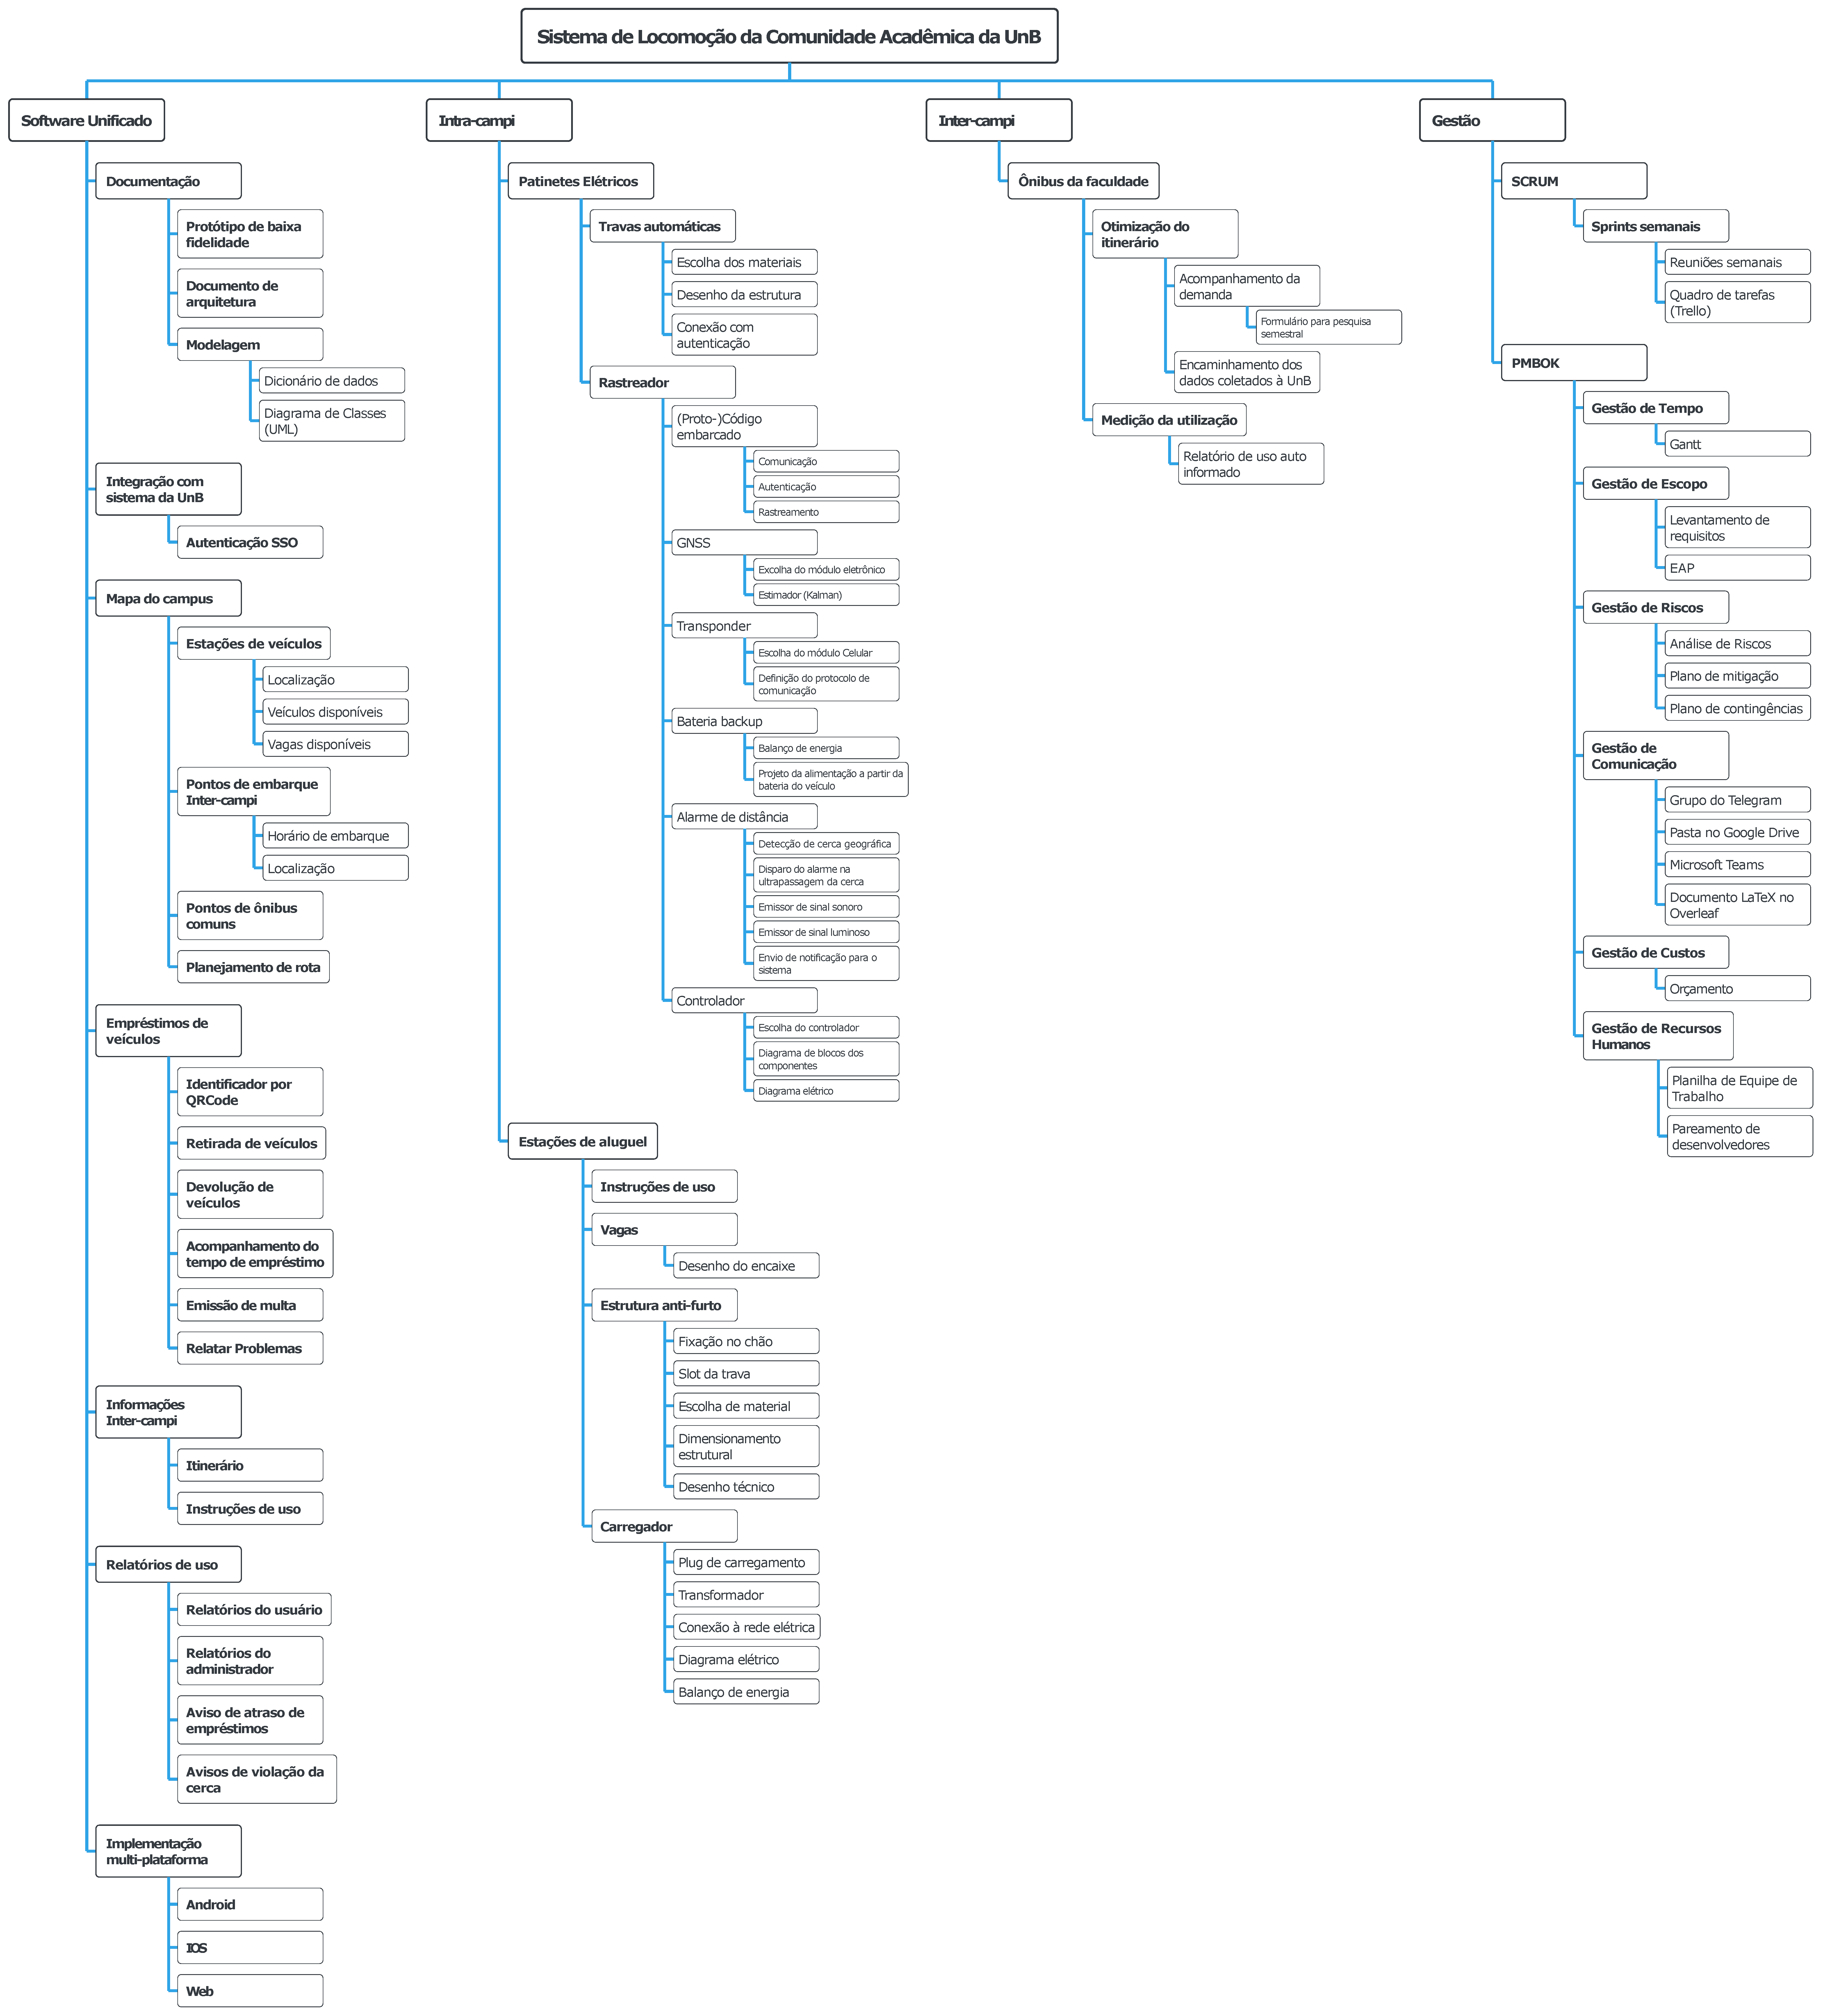
\includepdf[scale=0.8, pagecommand={}]{apendices/EAP.pdf}


\chapter{Diagrama Gantt}
\label{sec:Gantt}

\includepdf[landscape, scale=0.8, pagecommand={}]{apendices/cronograma.pdf}


\chapter{Protótipo de Baixa Fidelidade}
\label{sec:prototipoBaixa}

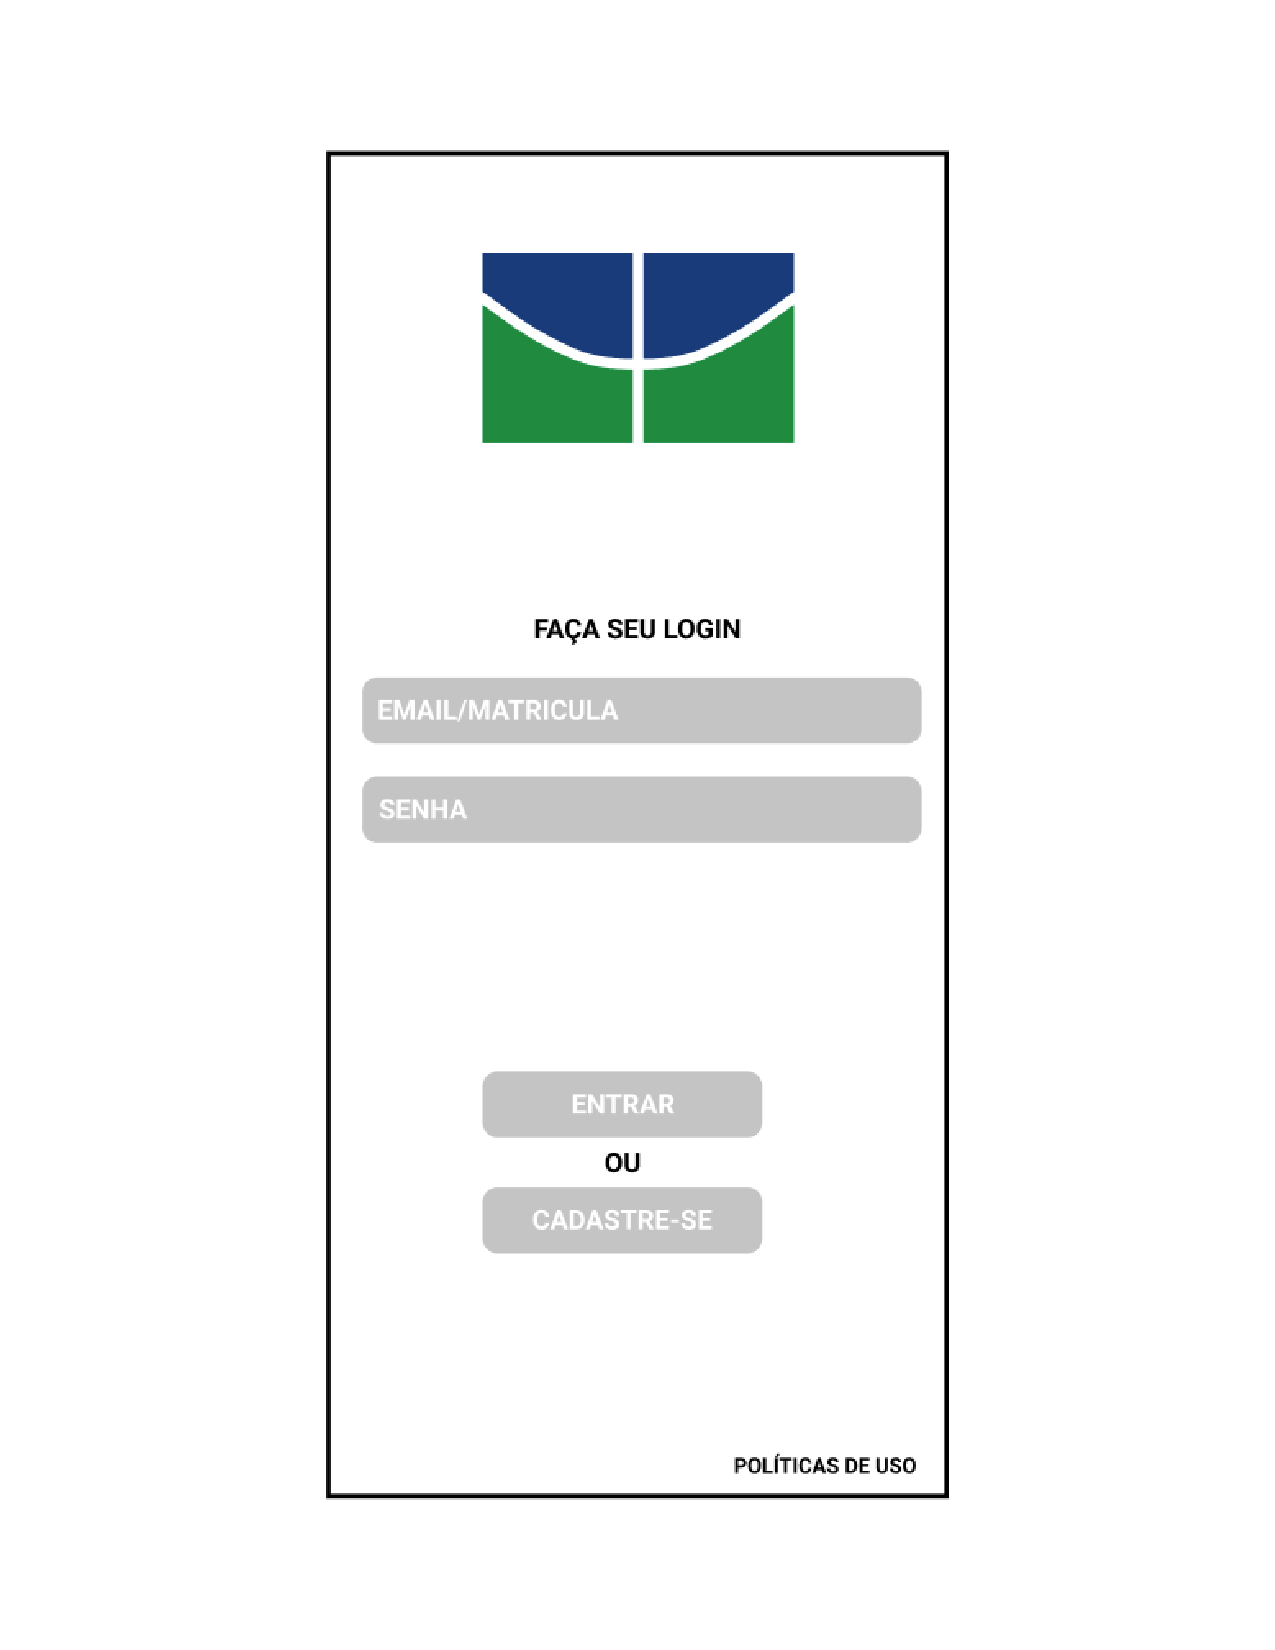
\includepdf[pages=-, nup=2x2, scale=0.9, pagecommand={}]{apendices/prot_lo_fi.pdf}


\end{apendicesenv}

% Anexos
% \begin{anexosenv}
% \partanexos

% % \input{editaveis/12_anexos}

% \end{anexosenv}

% Índice remissivo
\printindex


\end{document}